
    Figure~\ref{reord:cond_counter_example1(a)} shows an example of a program with conditionals(left) along with with its candidate execution(right) where the case of outcome in the red box is not possible. 
    \begin{figure}[H]
        \centering 
        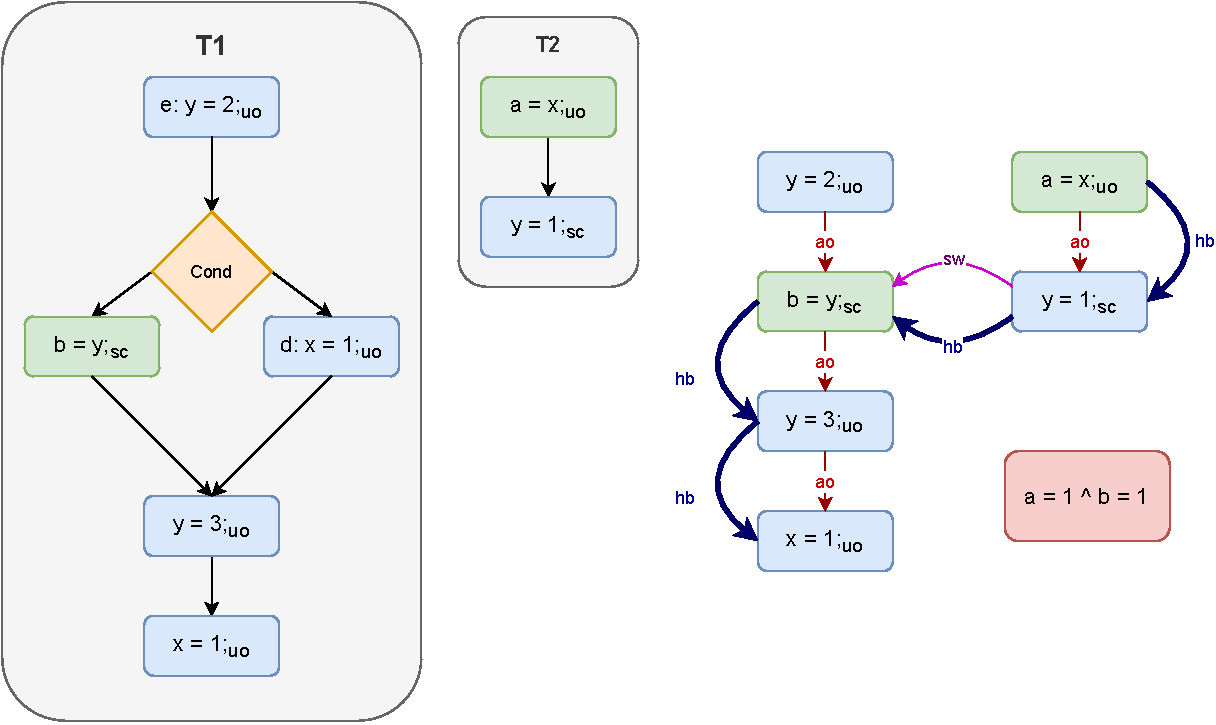
\includegraphics[scale=0.7]{7.CounterExamples/ReorderingConditionals/CounterExamples1a(Conditionals).pdf}
        \caption{Case with conditionals where $a = 1, b = 1$ is invalid due to Coherent Reads.}
        \label{reord:cond_counter_example1(a)}
    \end{figure}
    
    Observations:
    \begin{itemize}
        \item From the Candidate Execution, we can infer $\reln{\{a=x;_{uo}\}}{hb}{\reln{\{y=1;_{sc}\}}{hb}{\reln{\{b=y;_{sc}\}}{hb}{\reln{\{y=3;_{uo}\}}{hb}{\{x=1;_{uo}\}}}}}$.
        \item By Axiom \ref{CoRe}, the read $a$ cannot have value of $x$ read as $1$. 
        \item This inference was due to $\reln{\{a=x;_{uo}\}}{hb}{\{x=1;_{uo}\}}$.
    \end{itemize}
    
    Figure~\ref{reord:cond_counter_example1(b)} shows the program after reordering(right) two writes in $T1$ along with its candidate execution(left) where the case of reads in the orange box is possible\footnotemark. 
    \begin{figure}[H]
        \centering 
        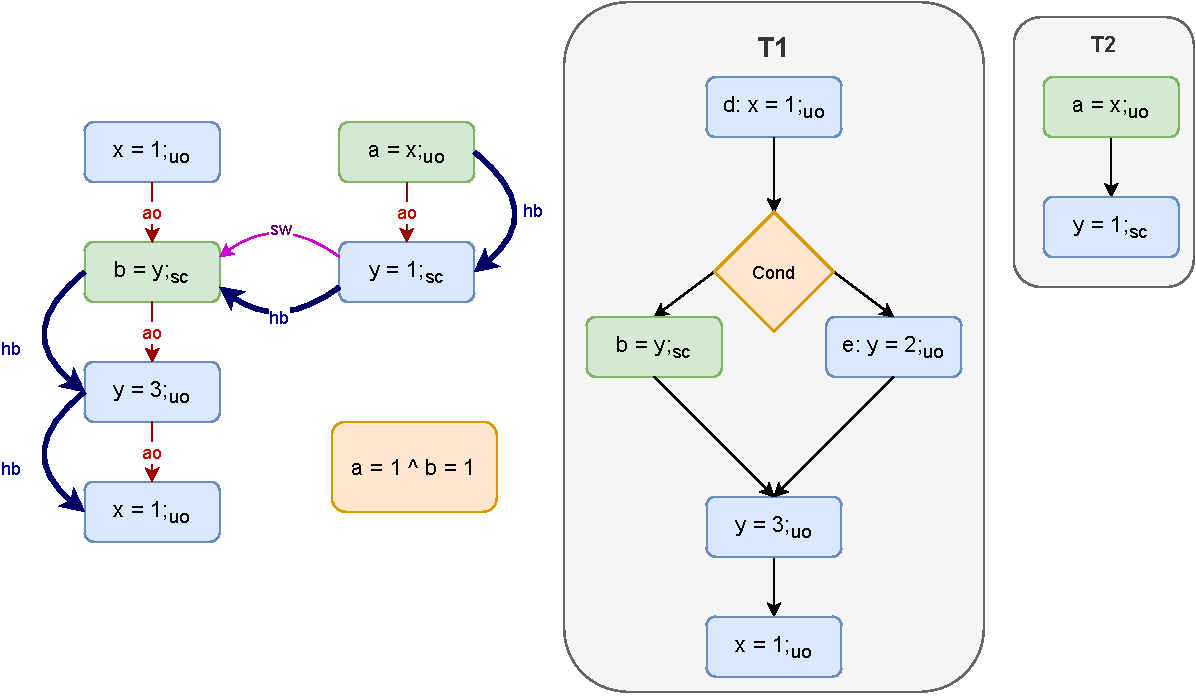
\includegraphics[scale=0.7]{7.CounterExamples/ReorderingConditionals/CounterExamples1b(Conditionals).pdf}
        \caption{Case where events of T1 are reordered, resulting in $a = 1,  b = 1$ to be valid.}
        \label{reord:cond_counter_example1(b)}
    \end{figure}
    
    \footnotetext{Notice that the above counterexample can also be justified by introducing a new write $x=1$ in a candidate.}
    Observations:
    \begin{itemize}
        \item From the Candidate Execution, we can infer $\reln{\{a=x;_{uo}\}}{hb}{\{x=1;_{uo}\}}$. 
        \item But there is no $\stck{_{hb}}$ relation with event $d$ and the read to $x$, i.e. $\neg \reln{\{a=x;_{uo}\}}{hb}{d:\{x=1;_{uo}\}}$
        \item No Axiom restricts the read $a$ to have value of $x$ as $1$.
    \end{itemize}
    
    Figure~\ref{reord:cond_counter_example2(a)} shows an example of a program(left) with 1-branch conditional along with with its candidate execution(right) where the case of outcome in the red box is not possible. 
    \begin{figure}[H]
        \centering 
        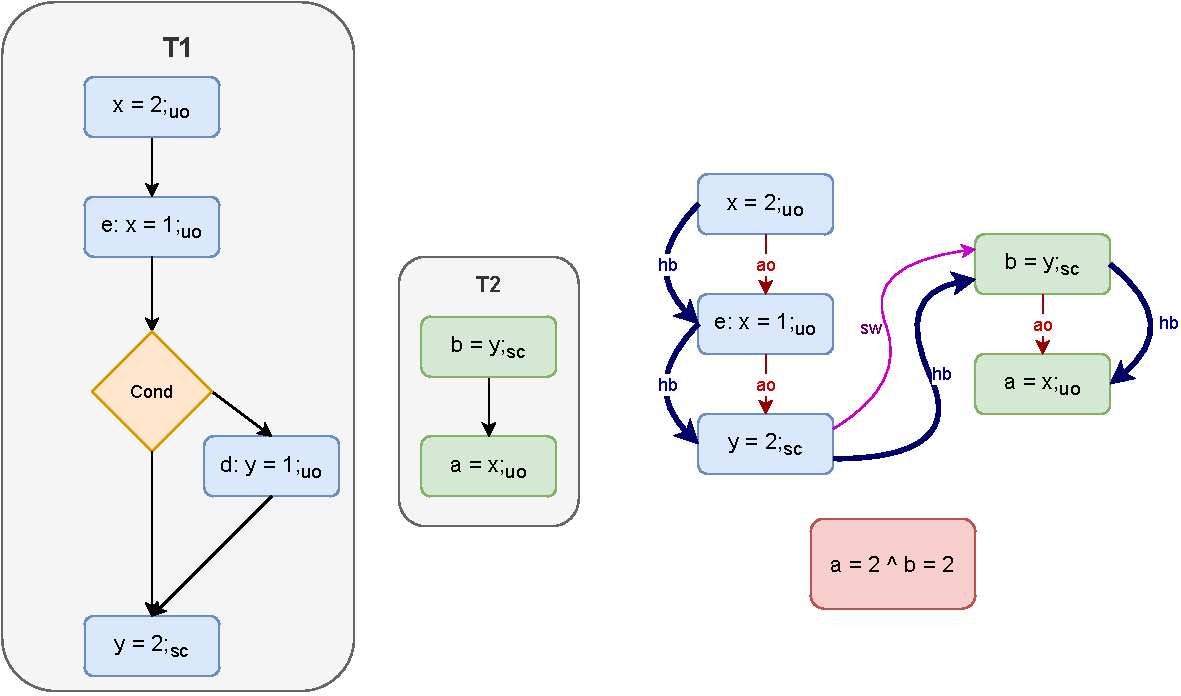
\includegraphics[scale=0.7]{7.CounterExamples/ReorderingConditionals/CounterExamples2a(Conditionals).pdf}
        \caption{Case with conditionals where $a = 2, b = 2$ is invalid due to Coherent Reads.}
        \label{reord:cond_counter_example2(a)}
    \end{figure}
    
    Observations:
    \begin{itemize}
        \item From the Candidate Execution, we can infer $\reln{\{x=2;_{uo}\}}{hb}{\reln{\{x=1;_{uo}\}}{hb}{\reln{\{y=2;_{sc}\}}{hb}{\reln{\{b=y;_{sc}\}}{hb}{\{a=x;_{uo}\}}}}}$.
        \item By Axiom \ref{CoRe}, the read $a$ cannot have the value of $x$ to be read as $2$.  
        \item This inference was due to the relation $\reln{\{x=2;_{uo}\}}{hb}{\reln{\{x=1;_{uo}\}}{hb}{\{a=x;_{uo}\}}}$.
    \end{itemize}
    
    Figure~\ref{reord:cond_counter_example2(b)} shows the program after reordering(right) two writes in $T1$ along with its candidate execution(left) where the case of reads in the orange box is possible\footnotemark. 
    \begin{figure}[H]
        \centering 
        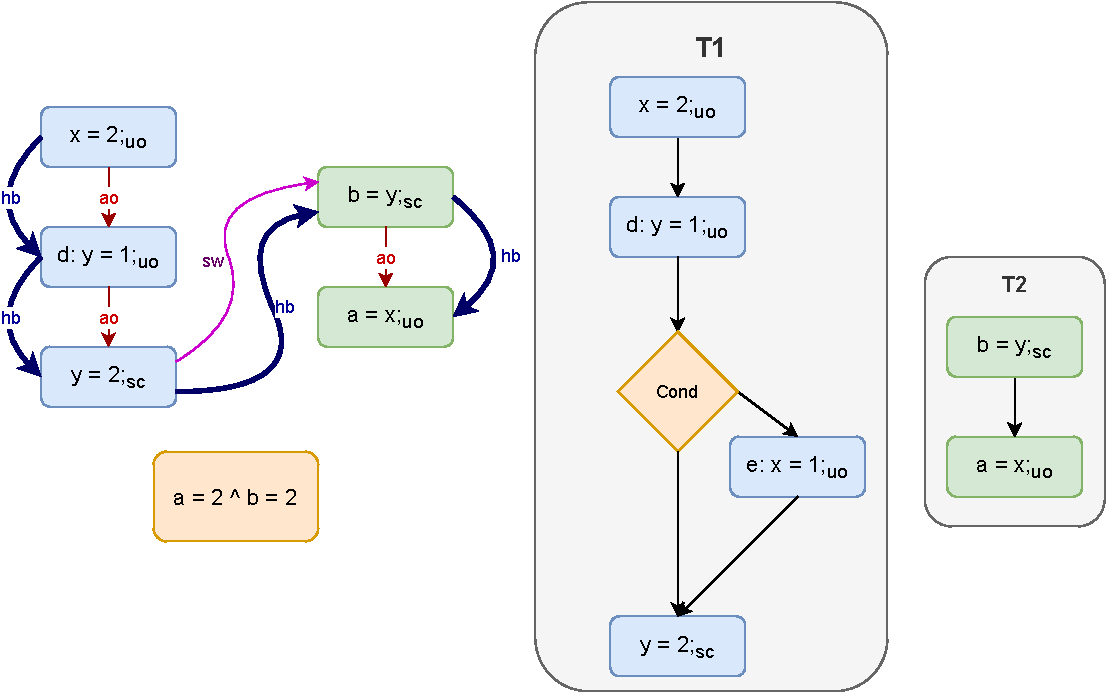
\includegraphics[scale=0.7]{7.CounterExamples/ReorderingConditionals/CounterExamples2b(Conditionals).pdf}
        \caption{Case where events of $T1$ are reordered, resulting in $a = 2,  b = 2$ to be valid.}
        \label{reord:cond_counter_example2(b)}
    \end{figure}

    \footnotetext{Notice that the above counterexample can also be attributed to the elimination of a write $x=1$.}
    Observations:
    \begin{itemize}
        \item From the Candidate Execution, we can infer $\reln{x=1;_{uo}}{hb}{a=x;_{uo}}$. 
        \item But there is no $\stck{_{hb}}$ relation with event $e$ and the read to $x$, i.e. $\neg \reln{e:x=1;_{uo}}{hb}{a=x;_{uo}}$.
        \item No Axiom restricts the read $a$ to have value of $x$ as $2$.
    \end{itemize}
%-----------------------------------------------------------------------------------------------------------------------------------
    We leave the rest of the cases as an exercise to the avid reader\footnotemark.

    \footnotetext{While showing reordering of reads, one must note that the introduction of new observable behaviors is dependant on the fact that a candidate execution has a local variable which must have not been there because the conditional branch was not taken. Note that this fact does not rely on the consistency rules of the memory model. It could be the case that the compiler instantiates the local variables to some default value (say 0), and then decides to reorder a read outside a conditional on the assertion that the read of local variable will return the same constant value. Having such an assertion in general might not be always certain. This is one of the main drawbacks of not using information as to why the compiler would do such a transformation.}
%------------------------------------------------------------------------------------------------------------------------------------------